\chapter{Introduzione}
\section{Gestione dei dati tramite Use Case}
Nella gestione dei dati non sempre è sufficiente un database relazionale soprattutto
quando si hanno tanti dati e tanti utenti in accesso.

Nella gestione dobbiamo tenere traccia dei workload, carichi di lavoro che dipendono da:
\begin{itemize}
    \item letture/scritture
    \item numero di operazioni
    \item complessità delle operazioni
\end{itemize}
Un altro aspetto importante sono i volumi dei dati e l'eterogeneità.

Quando si trattano i dati si ha una pipeline di lavoro (value chain) composta da
tre fasi:
\begin{itemize}
    \item \textbf{Data discovery}: ottenimento, preparazione e organizzazione
          dei dati da diverse fonti
    \item \textbf{Data integration}: integrazione di tutti i dati provenienti da
          diverse fonti
    \item \textbf{Data exploitation}: analisi dei dati, visualizzazione e presa
          di decisione (studio esplorativo).
\end{itemize}
Per queste operazioni esistono differenti prodotti.
\begin{figure}[ht]
    \centering
    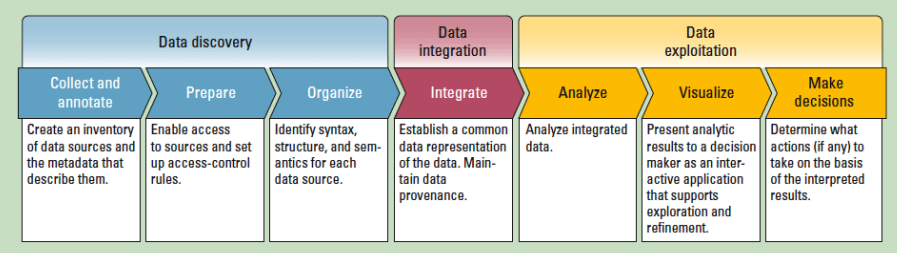
\includegraphics[width=0.8\textwidth]{./img/data_chain.png}
    \caption{Data value chain}
    \label{fig:valChain}
\end{figure}

L'obiettivo del corso è quello di progettare un'architettura dati in base al
contesto. Conoscere le tipologie di prodotti, nuovi modelli DBMS e gestione dei
dati.

Tutto si basa sugli Use Case
\begin{itemize}
    \item \textbf{Caso Bancario}: un'architettura dati che permetta di effettuare
          le normali operazioni bancarie. Questo consiste nella progettazione di
          un sistema distribuito relazionale (diversi database distribuiti), che
          gestisce interrogazioni e transazioni distribuite.
    \item \textbf{Machine Learning}: realizzazione di una pipeline per la
          costruzione dei dataset di training per addestrare modelli di ML.
          DAta centric AI, MLops.
    \item \textbf{Modelli e architetture non relazionali}: ne sono un esempio
          le API che restituiscono dati in formato JSON. Comprendono quindi
          modelli key-value, grafi, sistemi distribuiti relazionali ecc...
    \item \textbf{Cloud}: Utilizzo di sistemi di gestione dei dati in cloud,
          firebase e elastic search.
    \item \textbf{AI generativa per la gestione dei dati}: come usare AI
          generativa nei sistemi di gestione dei dati.
\end{itemize}
% Sistemo appena carica le slide
\section{Gestione operazioni bancarie}
Si vuole un'architettura dati che permetta di effettuare le normali operazioni
bancarie. La banca avrà $3$ sedi e dobbiamo progettare una base di dati efficiente 
e sicura.

Servirà la progettazione di sistemi distribuiti relazionali (diversi
database distribuiti), interrogazioni distribuite e transazioni distribuite.

Abbiamo le seguenti operazioni:
\begin{itemize}
    \item transazioni bancarie
    \item bonifici multibanca
\end{itemize}
Per prima cosa bisogna studiare il workload:
\begin{itemize}
    \item letture e scritture: bilanciate
    \item quante sono: sono tante
    \item complessità: semplici
\end{itemize}
I volume dei dati è elevato

Si ha eterogeneità dei sistemi.

Bisogna stare attenti agli update che devono essere veloci e consistenti.

L'architettura dati iniziale potrebbe essere centralizzata, in una regione, 
questo comporta notevoli problemi di sicurezza e tempi di accesso alti. 

L'architettura di base non è più sufficiente perché possiamo perdere i dati visto
che abbiamo un unico punto di fallimento. Soluzione: distribuzione del database
su più nodi.
\begin{figure}[!ht]
    \centering
    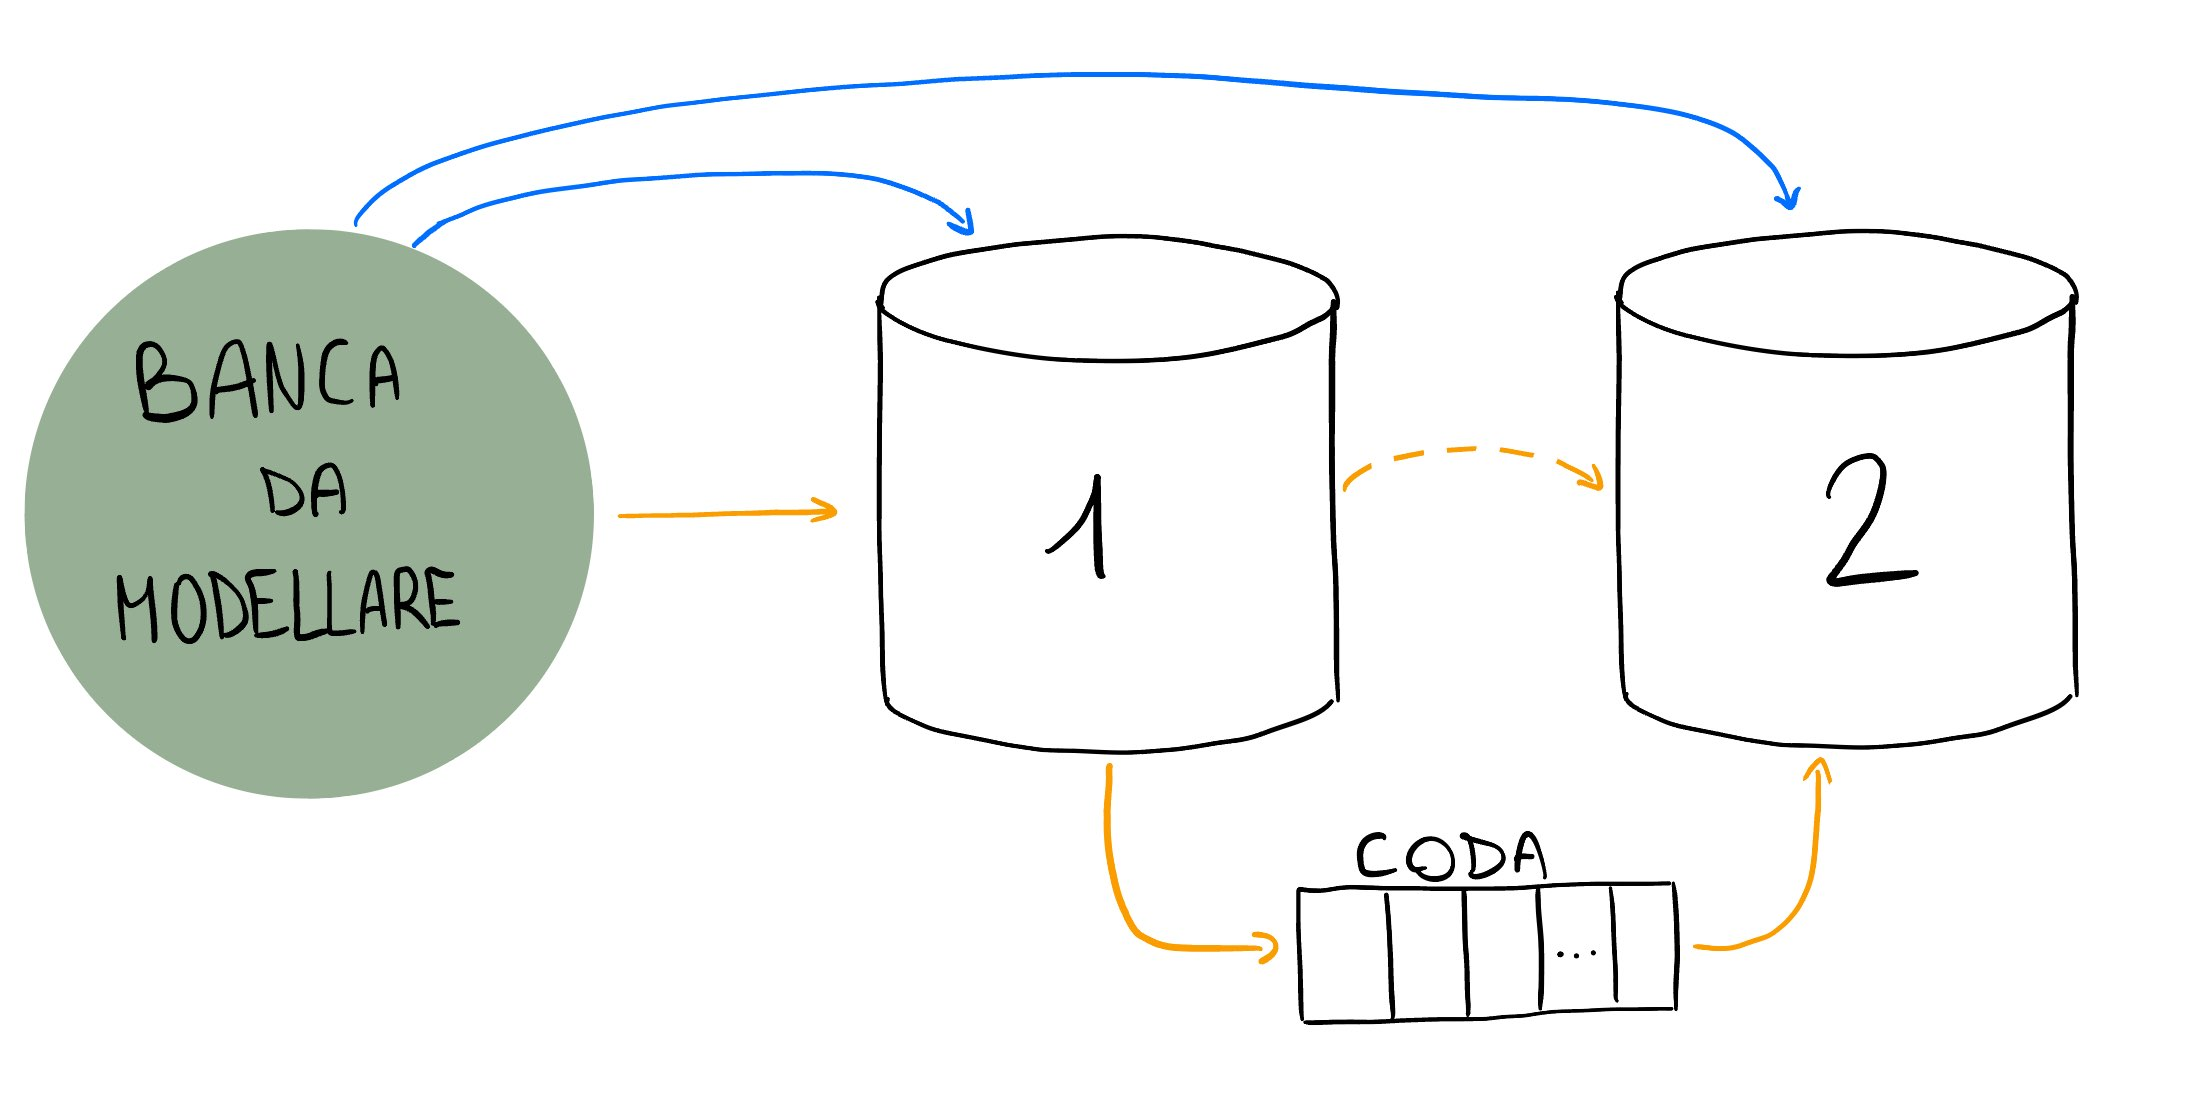
\includegraphics[width=0.8\textwidth]{./img/modellazione_banca.jpg}
    \caption{Architettura dati per update veloci e consistenti}
    \label{fig:esBanca}
\end{figure}

Un primo modo di distribuire i dati è effettuare una \textbf{replica} sulle altre 
sedi, questo tempi di scritture maggiorati, tempi per le letture ridotte e 
non abbiamo più un unico punto di fallimento. L'implementazione della replica può
essere fatta in diversi modi. Nella figura \ref{fig:esBanca} si possono notare due 
esempi di soluzioni identificate dai colori delle frecce blu e arancioni:
\begin{itemize}
    \item \textbf{Blu}: la prima soluzione proposta comprende il salvataggio
          dei dati su due memorie posizionate in luoghi differenti. Questo approccio è più
          semplice a discapito della velocità, perché dobbiamo scrivere su entrambi,
          ma possiamo leggere solo da una.
    \item \textbf{Arancione}: nella seconda proposta si utilizza un approccio
          master-slave, dove inizialmente si effettua un salvataggio solo su una
          prima memoria. Lo step successivo è sfruttare i log per replicare i
          dati sulla seconda. Dal momento che la quantità dei dati è elevata,
          si può aggiungere un middleware (coda) che permette di mantenere la
          consistenza tra le due parti. In questo approccio più complesso si
          dovrà anche gestire la frequenza di aggiornamento dei dati della
          memoria secondaria. Quando uno dei due cade allora ci si adopera per
          spostare il carico sull'altro nodo. Un problema di questa soluzione è 
          capire quando allineare le repliche. Se volessimo avere la corretta 
          lettura su ciascuna replica allora dobbiamo allinearle ogni volta che 
          scriviamo sul master, oppure possiamo leggere tutte le repliche e 
          considerare solo l'informazione presente su più repliche (majority base)
\end{itemize}
%la parte qui sotto non andrebbe messa con la spiegazione che ci aveva fatto a 
% fine lezione? È più un esempio del DDBMS
Nel nostro use case, per implementare una base di dati di una banca dobbiamo ragionare
prima sui vincoli introdotti dalla legge, la quale afferma che bisogna avere i
dati dislocati in almeno $3$ regioni geografiche diverse. Perciò non possiamo più
ragionare sul centralizzato ma dobbiamo parlare di distribuito.

Possiamo avere $3$ sedi dislocate geograficamente, il nodo di Milano ha la logica
applicativa mentre a Roma e Padova ho solo l'applicazione, i dati saranno in tutte
e tre le regioni.

Avendo $3$ sedi distaccate in cui vengono salvati i dati, bisogna capire cosa salvare
e dove salvarlo.
Una \textbf{prima soluzione} è salvare tutto in tutte e tre le regioni (replica), 
questo comporta maggior tempo per effettuare le scritture, con un vantaggio nella 
velocità di lettura.

La \textbf{seconda soluzione} è salvare i dati solo nella regione dove vengono 
utilizzati, questo significa \textbf{frammentare} i dati. Ex: Roma c'è il
reparto risorse umane allora i dati sulle risorse umane verranno spostati lì.

Ovviamente si possono avere dati utili per più sedi, la soluzione è salvarli in
entrambe le sedi (replica).
\begin{nota}
    La frammentazione porta vantaggi nelle letture e scritture a patto che non
    si facciano operazioni su dati non in comune tra sedi. In caso contrario si
    hanno gli stessi problemi della prima soluzione.
\end{nota}
\begin{nota}
    Distribuire i dati è molto complesso e rischioso, conviene farlo solo quando 
    è davvero necessario prima di aggiungere complessità inutilmente. Motori di 
    database distribuiti, frammentare i dati tra nodi diversi, oppure edge 
    computing i device salvano localmente i dati. Il problema è che quando si 
    distribuiscono i dati bisogna capire cosa distribuire, ovvero capire come 
    distribuire tra client e server le parti di gestione.
\end{nota}
